\section{闭环数值验证、机理分解与虚拟物理验证}\label{sec:experiments}

\subsection{实验设置、外部对比基线与统计评价指标}
本节在密集三角晶格位置互换与随机全排列基准上，系统评估所提包络等变图策略与邻域近端分配协同控制方法（EGP-NPA）在训练规模（$N=8$）与跨规模零样本迁移（$N\in\{12,20,25\}$）下的任务完成率、收敛效率、三部件协同机理及消融特性。全部实验采用统一物理与安全参数：安全避碰距离 $\ds=1.000\ \mathrm m$，单机速度上限 $U=0.50\ \mathrm{m/s}$，工作区边界 $B_{\mathrm{ws}}=4.0\ \mathrm m$，多项式信道截断半径 $R_c=10.0\ \mathrm m$，一跳感知与通信半径 $R_{\mathrm{sense}}=2.50\ \mathrm m$，障碍函数衰减率 $\alpha_c=\alpha_s=\alpha_x=2.0\ \mathrm s^{-1}$，标称采样步长 $\Delta t=0.05\ \mathrm s$，最大物理时域 $T_{\max}=60.0\ \mathrm s$。初始构型为相邻间距 $1.001\ \mathrm m$（初始接触净空仅 $1.0\ \mathrm{mm}$）的紧密三角晶格阵列。图\ref{fig:train-curves}展示了训练期（$9.6\times 10^5$ 环境步）回合累积奖励与 $N=8$ 验证集确定性达标率的演化曲线：初始零残差策略（等价于短视比例吸引控制）在验证集上的达标率仅为 $19.4\%$，而 EGP-NPA 在约 $5.0\times 10^5$ 步后稳定收敛至 $100\%$ 验证达标率。

\begin{figure*}[t]
 \centering
 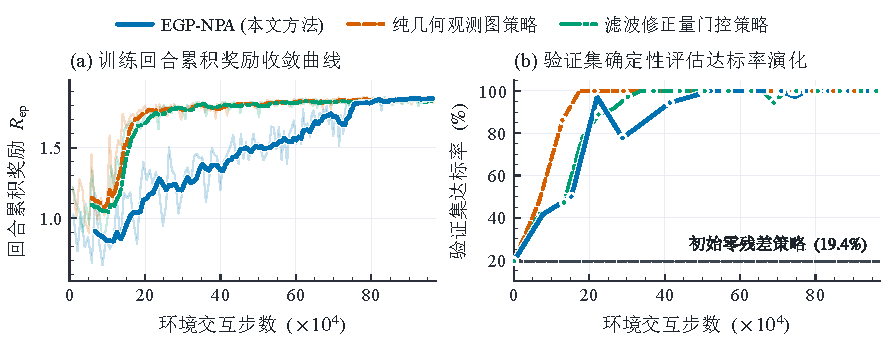
\includegraphics[width=\textwidth]{figures_zh/fig2_training_curves.pdf}
 \caption[MAPPO 训练回合累积奖励与验证集确定性评估达标率收敛曲线]{多智能体近端策略优化（MAPPO）训练过程演化对比。(a) 训练回合累积奖励 $R_{\mathrm{ep}}$ 收敛曲线（浅色细线为原始回合回报，深色粗线为滑动平均）；(b) 验证集（$N=8$，$36$ 组标准互换与全排列场景）确定性评估达标率演化曲线。}
 \label{fig:train-curves}
\end{figure*}

\begin{table*}[t]
 \centering\footnotesize
 \caption{训练规模基准（$N=8$，两档连通阈值各 $32$ 组实例）上 EGP-NPA 与三类安全强化学习方法及两类经典基线的闭环对比统计}\label{tab:e1}
 \begin{tabularx}{\textwidth}{@{}Xcccccc@{}}
 \toprule
 控制方法 & $f=0.60$ 达标率 & $f=0.60$ 中位时间 & $f=0.90$ 达标率 & $f=0.90$ 中位时间 & 证书步长减半 & 有理数审计违约\\
 \midrule
 \textbf{EGP-NPA（本文方法）} & $\mathbf{32/32\ (100\%)}$ & $\mathbf{7.32\ \mathrm s}$ & $\mathbf{32/32\ (100\%)}$ & $\mathbf{7.12\ \mathrm s}$ & $\mathbf{0}$ & $\mathbf{0}$\\
 护盾投影一致性强化学习\cite{wabersich2021,liu2026saferl}（Proj-MAPPO + NPA，$B=8$） & $32/32\ (100\%)$ & $9.53\ \mathrm s$ & $32/32\ (100\%)$ & $10.73\ \mathrm s$ & $0$ & $0$\\
 去中心化静态 CBF 护盾图策略\cite{zhang2025gcbf,zhang2025dgppo}（Static-CBF GNN，$B=0$） & $5/32\ (15.6\%)$ & $13.30\ \mathrm s$ & $6/32\ (18.8\%)$ & $13.88\ \mathrm s$ & $431\,725$ & $0$\\
 拉格朗日约束强化学习\cite{gu2023safe}（MAPPO-Lagrangian，无硬护盾） & $0/32^\ddagger\ (0\%)$ & $4.15\ \mathrm s^\ddagger$ & $0/32^\ddagger\ (0\%)$ & $4.15\ \mathrm s^\ddagger$ & --- & $7\,029$\\
 Gon\c{c}alves 等\cite{goncalves2023circulation}切向环流启发式 + 动态分摊 ($B=8$) & $21/32\ (65.6\%)$ & $32.50\ \mathrm s$ & $18/32\ (56.3\%)$ & $30.50\ \mathrm s$ & $0$ & $0$\\
 Ames 等\cite{ames2017cbf,reis2021}短视比例吸引滤波 + 动态分摊 ($B=8$) & $17/32\ (53.1\%)$ & $36.35\ \mathrm s$ & $16/32\ (50.0\%)$ & $31.80\ \mathrm s$ & $0$ & $0$\\
 切向环流启发式 + 静态配额平摊滤波\cite{ames2017cbf,zhang2025gcbf} ($B=0$) & $2/32\ (6.3\%)$ & $25.10\ \mathrm s$ & --- & --- & $72\,156$ & $0$\\
 \bottomrule
 \end{tabularx}
 \vspace{1.5pt}
 \par\raggedright\scriptsize 注：$^\ddagger$\texttt{MAPPO-Lagrangian} 名义轨迹虽在 $64/64$ 组实例中到达目标邻域（中位时间 $4.15\ \mathrm s$），但全部 $64$ 组运行均发生严重碰撞安全违约（合计 $7\,029$ 个违约保持段，中位最小机间距离 $0.263\ \mathrm m < \ds=1.000\ \mathrm m$），故无违约安全达标数为 $0/32$。
\end{table*}

主评测基准包含两类共 $96$ 组独立随机初值实例：
\begin{enumerate}
 \item \textbf{训练规模基准（$N=8$，共 $64$ 组实例）：} 含 $20$ 组局部成对互换（$1\sim 3$ 对相邻节点互换目标，其余节点目标在原地）与 $12$ 组随机全排列任务，分别在常规连通阈值 $f=\lr/\lambda_2(\bp_0)=0.60$（$32$ 组）与紧连通阈值 $f=0.90$（$32$ 组）下评测。
 \item \textbf{跨规模零样本迁移基准（$N\in\{12,20,25\}$，共 $32$ 组实例）：} 包含 $N=12$（$12$ 组：含 $8$ 组局部互换与 $4$ 组全排列）、$N=20$（$12$ 组：含 $8$ 组局部互换与 $4$ 组全排列）与 $N=25$（$8$ 组局部互换），连通阈值比例取 $f=0.60$。学习控制律直接复用小规模（$N\in\{6,\dots,10\}$，验证规模 $N=8$）训练所得的图网络参数 $\theta^\star$ 进行零样本部署。
\end{enumerate}

在主对比实验中，将所提 EGP-NPA 与\textbf{三类代表性安全强化学习方法}及\textbf{三类经典解析/启发式安全控制基线}进行综合对比：
\begin{enumerate}
 \item \textbf{护盾投影一致性安全强化学习（\texttt{Proj-MAPPO + NPA}\cite{wabersich2021,liu2026saferl}）：} 代表近期将安全滤波器干预量作为正则惩罚反馈给策略网络的预测/自适应安全强化学习范式。采用与本文完全相同的两层等变 GNN、闭邻域完成包络 $\rho_{i,k}$ 与 $B=8$ 闭邻域块 NPA 护盾，但在策略训练损失中加入护盾投影一致性正则项 $\mathcal L_{\mathrm{proj}}(\theta)=\lambda_{\mathrm{proj}}\frac1N\sum_{i=1}^N\norm{\Pi_{\mathcal U_i}(\bu_{i,k}^{\mathrm{nom}}(\theta))-\operatorname{sg}(\bu_{i,k})}_2^2$（按梯度范数比标定权重 $\lambda_{\mathrm{proj}}=1.0$），引导标称策略贴合安全滤波输出以降低滤波干预；
 \item \textbf{去中心化静态 CBF 护盾图策略（\texttt{Static-CBF GNN}，GCBF+/DGPPO 范式\cite{zhang2025gcbf,zhang2025dgppo}）：} 代表采用图神经网络策略配合单机独立/成对静态责任平摊 CBF-QP 护盾的分布式安全学习方法。采用等变 GNN 策略与完成包络 $\rho_{i,k}$，但底层安全滤波采用静态配额平摊（$B=0$，即固定 $s_{ia,k}\equiv 0$，无闭邻域块动态份额转移 $t_e$）；
 \item \textbf{原始—对偶拉格朗日安全强化学习（\texttt{MAPPO-Lagrangian}\cite{gu2023safe}）：} 代表无硬优化护盾的约束马尔可夫决策过程（CMDP）多智能体安全强化学习范式。采用相同两层等变 GNN 策略、任务价值网络与代价价值网络，将每拍碰撞与谱连通违约代价 $C_k=\sum_{i<j}(\ds+\delta_d-d_{ij,k+1})_++(\lr-\lambda_2(\bL(\bp_{k+1})))_+$ 通过对偶上升更新的拉格朗日乘子 $\lambda_{\mathrm{lag}}\ge 0$ 融入策略梯度目标；
 \item \textbf{经典解析与启发式安全控制基线：} 包括 Gon\c{c}alves 等\cite{goncalves2023circulation}的切向环流启发式控制（常值 $\omega_i\equiv 1,r_i\equiv 0,\psi_{ij}\equiv 0$ 配动态分摊 $B=8$）、Ames 等\cite{ames2017cbf,reis2021}的短视比例吸引安全滤波（$\bu_i^{\mathrm{nom}}=-\be_i$ 配动态分摊 $B=8$），以及切向环流配静态配额平摊滤波（$B=0$）。
\end{enumerate}
任务达标判据定义为全网最大目标误差 $\max_{i\in\mathcal V}\norm{\bp_i(t)-\bg_i}_2\le 0.01\ \mathrm m$ 并连续保持 $1.0\ \mathrm s$（达标时间取该窗口起始时刻；连续 $100$ 拍全网速度范数低于 $10^{-6}\ \mathrm{m/s}$ 记为零速死锁停滞）。每条闭环轨迹的全部零阶保持执行段均经受定理\ref{thm:zoh-safe}的精确有理数碰撞与谱下界审计（仅当全程有理数审计 $0$ 违约且满足达标判据时计为安全达标）。不同方法的安全达标率差异采用不一致对（Discordant Pairs）的双侧精确二项检验（McNemar 检验）评估显著性，并在共同达标实例上计算配对达标时间差中位数。

\subsection{代表性密集互换与全排列任务的闭环状态演化}
首先考察 $N=20$ 紧密三角晶格中的内部单对节点互换任务（中间 $2$ 台相邻机器人需互换位置，外围 $18$ 台辅助机器人初始已处于各自目标位置）。图\ref{fig:swap-traj}与图\ref{fig:time-evol}分别给出了空间运动轨迹、底层通信拓扑以及全网最大位置误差、物理图代数连通度 $\lambda_2(\bL(t))$、最小机间距离与均方根控制速度的时间演化响应。

\begin{figure*}[t]
 \centering
 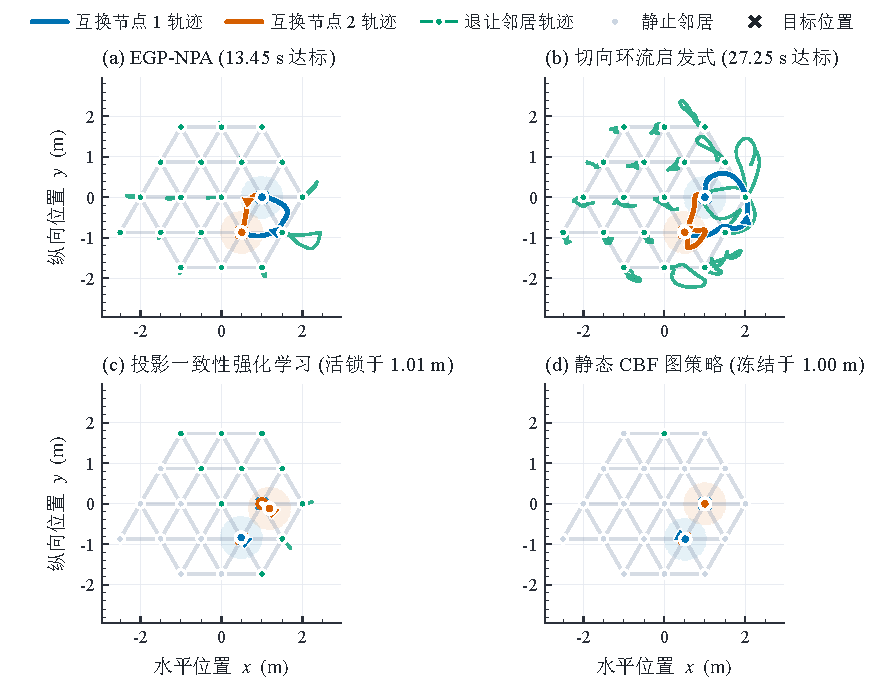
\includegraphics[width=\textwidth]{figures_zh/fig3_swap_trajectory.pdf}
 \caption[$N=20$ 密集晶格内部单对节点互换任务的空间运动轨迹与通信拓扑对比]{$N=20$ 密集晶格内部单对节点互换任务的空间运动轨迹与通信拓扑对比。(a) EGP-NPA 驱动待互换节点沿切向顺畅绕行，并通过闭邻域动态份额转移促使外围静止邻居（翠绿色回路）向外退让后归位，$13.45\ \mathrm s$ 达标；(b) Gon\c{c}alves 等\cite{goncalves2023circulation}的切向环流启发式引发外围多节点大范围旋转冲突，$27.25\ \mathrm s$ 达标；(c) 投影一致性安全强化学习（\texttt{Proj-MAPPO + NPA}\cite{wabersich2021,liu2026saferl}）因惩罚法向滤波修正量削弱了退让驱动 $\delta_n>0$，无法推开外圈静止邻居而活锁于 $1.01\ \mathrm m$；(d) 去中心化静态 CBF 护盾图策略（\texttt{Static-CBF GNN}\cite{zhang2025gcbf,zhang2025dgppo}，$B=0$）因静态配额平摊锁死外围静止邻居而冻结于 $1.00\ \mathrm m$。}
 \label{fig:swap-traj}
\end{figure*}

\begin{table*}[t]
 \centering\footnotesize
 \caption{跨规模零样本迁移基准（$N\in\{12,20,25\}$，共 $32$ 组实例）上 EGP-NPA 与三类安全强化学习方法及两类经典基线的对比统计}\label{tab:e2}
 \begin{tabularx}{\textwidth}{@{}Xccccccr@{}}
 \toprule
 控制方法 & $N=12$ ($12$ 组) & $N=20$ ($12$ 组) & $N=25$ ($8$ 组) & 总达标率 ($32$ 组) & 不一致对 ($p$ 值) & 中位 $\Delta t$ & 步长减半\\
 \midrule
 \textbf{EGP-NPA（本文方法）} & $\mathbf{12/12\ (6.52\ \mathrm s)}$ & $\mathbf{12/12\ (10.55\ \mathrm s)}$ & $\mathbf{8/8\ (10.43\ \mathrm s)}$ & $\mathbf{32/32\ (100\%)}$ & 基准 & 基准 & $\mathbf{0}$\\
 投影一致性强化学习\cite{wabersich2021,liu2026saferl}（Proj-MAPPO） & $9/12\ (17.25\ \mathrm s)$ & $5/12\ (17.70\ \mathrm s)$ & $3/8\ (12.30\ \mathrm s)$ & $17/32\ (53.1\%)$ & $15:0\ (6.1\times 10^{-5})$ & $-3.85\ \mathrm s$ & $0$\\
 静态 CBF 图策略\cite{zhang2025gcbf,zhang2025dgppo}（Static-CBF，$B=0$） & $0/12\ (\text{---})$ & $0/12\ (\text{---})$ & $1/8\ (19.85\ \mathrm s)$ & $1/32\ (3.1\%)$ & $31:0\ (9.3\times 10^{-10})$ & $-12.95\ \mathrm s$ & $447\,022$\\
 拉格朗日强化学习\cite{gu2023safe}（MAPPO-Lag.） & $0/12^\ddagger\ (4.05\ \mathrm s)$ & $0/12^\ddagger\ (3.95\ \mathrm s)$ & $0/8^\ddagger\ (3.92\ \mathrm s)$ & $0/32^\ddagger\ (0\%)$ & $32:0\ (4.7\times 10^{-10})$ & --- & $3\,900^\ddagger$\\
 Gon\c{c}alves 等\cite{goncalves2023circulation}切向环流启发式 & $7/12\ (14.40\ \mathrm s)$ & $4/12\ (24.53\ \mathrm s)$ & $2/8\ (38.22\ \mathrm s)$ & $13/32\ (40.6\%)$ & $19:0\ (3.8\times 10^{-6})$ & $-12.35\ \mathrm s$ & $14\,198$\\
 Ames 等\cite{ames2017cbf,reis2021}短视比例吸引滤波 & $4/12\ (34.30\ \mathrm s)$ & $1/12\ (55.50\ \mathrm s)$ & $0/8\ (\text{---})$ & $5/32\ (15.6\%)$ & $27:0\ (1.5\times 10^{-8})$ & $-26.70\ \mathrm s$ & $0$\\
 \bottomrule
 \end{tabularx}
 \vspace{1.5pt}
 \par\raggedright\scriptsize 注：前五种带护盾方法的有理数安全审计违约段数均为 $0$；$^\ddagger$\texttt{MAPPO-Lagrangian} 在全部 $32$ 组跨规模实例中均发生碰撞越界违约（最后一列记录其有理数审计违约段数 $3\,900$ 段，中位最小距离 $0.263\ \mathrm m<\ds$），故无违约安全达标率为 $0/32$。
\end{table*}

\begin{figure*}[t]
 \centering
 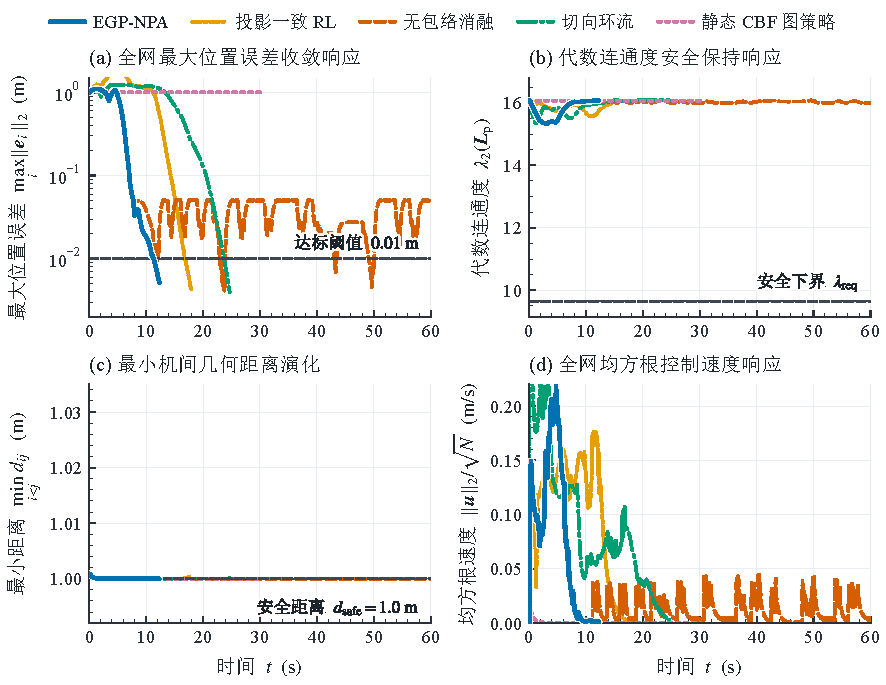
\includegraphics[width=\textwidth]{figures_zh/fig4_time_evolution.pdf}
 \caption[$N=20$ 内部互换任务中四项核心物理量的闭环时间响应对比]{$N=20$ 内部互换任务中四项核心物理量的闭环时间响应对比。(a) 全网最大位置误差 $\max_i\norm{\be_i(t)}_2$（对数坐标）；(b) 物理图代数连通度 $\lambda_2(\bL(t))$ 与安全下界 $\lr$；(c) 最小机间几何距离 $\min_{i<j}d_{ij}(t)$ 与安全距离 $\ds=1.0\ \mathrm m$；(d) 全网均方根控制速度 $\norm{\bu(t)}_2/\sqrt{N}$。}
 \label{fig:time-evol}
\end{figure*}

结合图\ref{fig:swap-traj}与图\ref{fig:time-evol}可以清晰观察到三项物理机制：
\begin{enumerate}
 \item \textbf{侧向破对称绕行与外围静止邻居的退让—归位闭环：} 在图\ref{fig:swap-traj}(d) 的去中心化静态 CBF 护盾图策略（\texttt{Static-CBF GNN}，$B=0$）下，由于外围 $18$ 台已处于目标位置的静止邻居拒绝让渡避碰份额，待互换节点的侧向绕行速度被单机半空间约束直接截断，全网均方根速度迅速跌至零（图\ref{fig:time-evol}(d) 紫色点线）；在图\ref{fig:swap-traj}(c) 的投影一致性安全强化学习（\texttt{Proj-MAPPO + NPA}）下，由于策略训练中惩罚了法向滤波修正量，待互换节点的法向切入分量 $\delta_n$ 过弱，无法推开双层包裹的外圈静止邻居而陷入原地小圈活锁（或在图\ref{fig:time-evol}(a) 另一初值下耗时 $16.90\ \mathrm s$ 缓慢达标）。而在图\ref{fig:swap-traj}(a) 的 EGP-NPA 下，等变图网络策略为蓝色与橙色节点生成充足的手性切向绕行推力，闭邻域动态分摊将该侧向压力通过接触边上的碰撞份额让渡传递给周围静止邻居，驱动紧邻的翠绿色节点走出紧凑的向外退让小回路以让出通道；待互换节点错身通过后，退让邻居在自身目标比例引力作用下平滑归位。
 \item \textbf{闭邻域完成包络对密集终点稳态悬停的精确消除：} 观察图\ref{fig:time-evol}(a) 与 (d) 中的朱砂橙色虚线（无完成包络消融）可见，虽然该模型在前 $8\ \mathrm s$ 内同样解开了内部互换死锁并将误差降至 $0.03\ \mathrm m$，但由于终点晶格间距 $1.001\ \mathrm m$ 紧贴安全阈值 $\ds=1.000\ \mathrm m$，接触对偶乘子持续非零使冲突门控保持常开，式\eqref{eq:nominal-law}中的零阶排斥偏置导致均方根速度在 $0.01\sim 0.04\ \mathrm{m/s}$ 之间持续脉动，最大误差卡在 $0.015\sim 0.05\ \mathrm m$ 形成稳态极限环。引入式\eqref{eq:envelope-def}的一跳闭邻域完成包络 $\rho_{i,k}$ 后，一旦闭邻域误差进入 $\varepsilon_g=0.05\ \mathrm m$ 球内，残差被一阶压灭（命题\ref{prop:envelope}），深海蓝色实线（EGP-NPA）直接穿过 $0.01\ \mathrm m$ 达标线并使控制速度归零。
 \item \textbf{全时域严格硬安全保持：} 如图\ref{fig:time-evol}(b)--(c) 所示，在整个穿插过程中，物理图代数连通度始终维持在 $\lambda_2(\bL(t))\ge 15.3 > \lr=9.69$，最小机间距离紧贴安全边界 $\ds=1.000\ \mathrm m$ 滑动而未发生任何越界。
\end{enumerate}

\subsection{与外部基线的训练规模及跨规模零样本迁移对比}
表\ref{tab:e1}与表\ref{tab:e2}分别汇总了 EGP-NPA 与三类代表性安全强化学习方法及两类经典安全控制基线在训练规模基准（$N=8$，$64$ 组实例）和跨规模零样本迁移基准（$N\in\{12,20,25\}$，$32$ 组实例）上的统计结果。对比数据揭示了四项清晰的定量结论：
\begin{enumerate}
 \item \textbf{无硬护盾约束强化学习（\texttt{MAPPO-Lagrangian}\cite{gu2023safe}）在毫米级净空晶格中必然发生安全违约：} 在初始接触净空仅 $1.0\ \mathrm{mm}$ 的密集三角晶格中，尽管 \texttt{MAPPO-Lagrangian} 通过对偶上升将拉格朗日乘子提升至 $\lambda_{\mathrm{lag}}=2.45$ 并在名义上于 $4.00\sim 4.15\ \mathrm s$ 内冲向目标，但软惩罚无法阻止多机相向对穿时的距离越界，在 $96$ 组场景上 $100\%$ 触发碰撞违约（合计 $10\,929$ 个违约保持段，安全达标率 $0\%$），直接证明了命题\ref{prop:safety}闭邻域硬安全护盾的必要性。
 \item \textbf{去中心化静态 CBF 护盾图策略（\texttt{Static-CBF GNN}\cite{zhang2025gcbf,zhang2025dgppo}，$B=0$）在大规模外圈包裹下失效：} 尽管该基线与 EGP-NPA 共享完全相同的等变 GNN 策略权重与终点包络，但由于底层采用单机静态责任平摊（$B=0$），外围目标点静止邻居拒绝退让，导致 $N=8$ 达标率仅为 $17.2\%$（$11/64$，触发 $431\,725$ 次步长减半），跨规模 $N\in\{12,20,25\}$ 达标率暴跌至 $3.1\%$（$1/32$，不一致对 $31:0,p=9.3\times 10^{-10}$），从闭环上证实了命题\ref{prop:unfreeze}第 1 款。
 \item \textbf{护盾投影一致性安全强化学习（\texttt{Proj-MAPPO + NPA}\cite{wabersich2021,liu2026saferl}）损害跨规模破死锁能力：} 在 $N=8$ 单层包裹晶格上，\texttt{Proj-MAPPO + NPA} 虽能实现 $64/64$ 达标，但中位达标时间（$9.53\ \mathrm s / 10.73\ \mathrm s$）比 EGP-NPA 慢 $2.88\ \mathrm s$；当零样本扩展至含多层静止邻居包裹的 $N\in\{12,20,25\}$ 阵列时，因投影一致性正则抑制了法向侵入驱动 $\delta_n>0$，其跨规模达标率降至 $53.1\%$（$17/32$，不一致对 $15:0,p=6.1\times 10^{-5}$，共同达标慢 $3.85\ \mathrm s$），严格印证了命题\ref{prop:unfreeze}关于法向推挤是触发配额让渡唯一动力源的理论分析。
 \item \textbf{相比经典解析/启发式基线的跨规模优势：} 随规模扩展至 $N=25$，Ames 等\cite{ames2017cbf,reis2021}短视滤波与 Gon\c{c}alves 等\cite{goncalves2023circulation}切向环流启发式的跨规模达标率分别降至 $15.6\%$（$27:0,p=1.5\times 10^{-8}$）与 $40.6\%$（$19:0,p=3.8\times 10^{-6}$）；而小规模（$N\le 10$）训练所得的 EGP-NPA 在全部 $96$ 组实例（含图\ref{fig:perm-gate}(a) 的 $20$ 机器人全排列穿插任务）上实现 $100\%$ 达标、零步长减半与零审计违约。
\end{enumerate}

\subsection{内部模块消融、动力学分解与独立盲测析因分析}\label{subsec:ablation}
表\ref{tab:decomp}汇总了三部分内部对照结果：（A）在 $32$ 组跨规模实例上移除闭邻域完成包络（$\rho_{i,k}\equiv 1$）以及不同训练输入/门控变体的跨规模统计；（B）在 $N=20$ 内部互换破死锁阶段（$t\in[0.05,1.00]\ \mathrm s$）相同 EGP-NPA 标称输入下动态分摊（$B=8$）与静态平摊（$B=0$）的执行速度分解；（C）固定 EGP-NPA 策略权重 $\theta^\star$ 在 $16$ 组跨规模实例上的执行期单变量门控替换与代数特征敲除统计（代表性响应见图\ref{fig:perm-gate}(b)）。

\begin{figure*}[t]
 \centering
 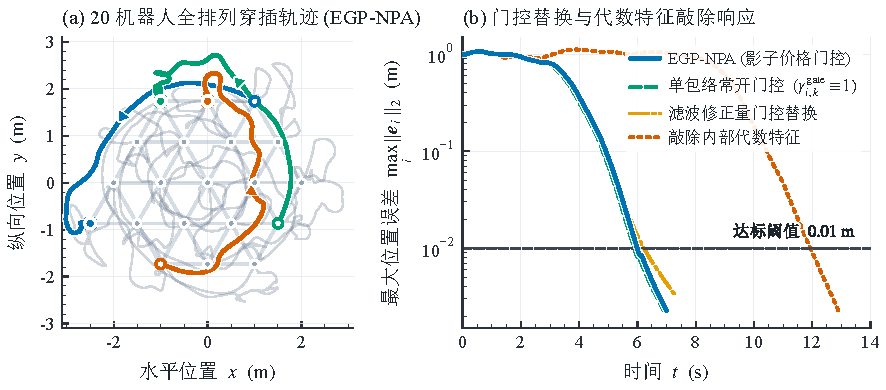
\includegraphics[width=\textwidth]{figures_zh/fig5_perm_and_gate.pdf}
 \caption[$20$ 机器人全排列穿插轨迹与固定权重下的门控替换及特征敲除响应]{$20$ 机器人全排列穿插轨迹与固定权重下的门控替换及特征敲除响应。(a) EGP-NPA 在 $N=20$ 随机全排列任务中的空间穿插轨迹（冷灰细线为背景群体轨迹，彩色实线突出显示三台大跨度对穿节点）；(b) 固定 EGP-NPA 策略权重 $\theta^\star$ 不变，在执行期分别采用原配影子价格门控 $\gamma^{\mathrm{gate},\mu}$、单包络常开门控 $\gamma^{\mathrm{gate}}\equiv 1$、滤波修正量门控 $\gamma^{\mathrm{gate,int}}$ 以及敲除内部代数特征时的误差收敛响应。}
 \label{fig:perm-gate}
\end{figure*}

\begin{table*}[t]
 \centering\footnotesize
 \caption{EGP-NPA 内部模块跨规模消融（A 部，$32$ 组实例）、破死锁阶段速度分解（B 部，$t\in[0.05,1.00]\ \mathrm s$）与固定权重 $\theta^\star$ 下的执行期单变量干预统计（C 部，$16$ 组实例）}\label{tab:decomp}
 \begin{tabularx}{\textwidth}{@{}Xccccr@{}}
 \toprule
 A. 内部模块跨规模消融（$32$ 组实例） & $N=12$ ($12$ 组) & $N=20$ ($12$ 组) & $N=25$ ($8$ 组) & 总达标率 ($32$ 组) & 不一致对 ($p$ 值) / 中位 $\Delta t$\\
 \midrule
 \textbf{EGP-NPA（完整架构）} & $12/12\ (6.52\ \mathrm s)$ & $12/12\ (10.55\ \mathrm s)$ & $8/8\ (10.43\ \mathrm s)$ & $\mathbf{32/32\ (100\%)}$ & 基准\\
 无完成包络消融（固定 $\theta^\star$，令 $\rho_{i,k}\equiv 1$） & $12/12\ (9.78\ \mathrm s)$ & $5/12\ (36.75\ \mathrm s)$ & $8/8\ (14.10\ \mathrm s)$ & $25/32\ (78.1\%)$ & $7:0\ (0.0156)$ / $-2.40\ \mathrm s$\\
 纯几何观测图策略（移除代数特征训练检查点） & $12/12\ (7.57\ \mathrm s)$ & $7/12\ (21.90\ \mathrm s)$ & $3/8\ (19.65\ \mathrm s)$ & $22/32\ (68.8\%)$ & $10:0\ (0.0020)$ / $-0.45\ \mathrm s$\\
 滤波修正量门控策略（$\gamma_{i,k}^{\mathrm{gate,int}}$ 训练检查点） & $10/12\ (11.20\ \mathrm s)$ & $4/12\ (30.08\ \mathrm s)$ & $1/8\ (6.80\ \mathrm s)$ & $15/32\ (46.9\%)$ & $17:0\ (1.5\times 10^{-5})$ / $-0.50\ \mathrm s$\\
 \midrule
 \multicolumn{4}{@{}l}{B. 相同 EGP-NPA 标称输入下的破死锁速度分解（$N=20$ 内部互换，$t\in[0.05,1.00]\ \mathrm s$）} & 动态分摊 ($B=8$) & 静态平摊 ($B=0$)\\
 \midrule
 \multicolumn{4}{@{}l}{待互换节点切向（侧向）标称速度均值 $|\hat{\be}_i^{\top}\bJ^{\top}\bu_i^{\mathrm{nom}}|$} & $0.8887\ \mathrm{m/s}$ & $0.8887\ \mathrm{m/s}$\\
 \multicolumn{4}{@{}l}{待互换节点切向（侧向）实际执行速度均值 $|\hat{\be}_i^{\top}\bJ^{\top}\bu_i|$} & $\mathbf{0.2003\ \mathrm{m/s}}$ & $0.0004\ \mathrm{m/s}$\\
 \multicolumn{4}{@{}l}{外围一跳静止邻居向中心外侧的标称残差速度均值} & $-0.0105\ \mathrm{m/s}$ & $-0.0105\ \mathrm{m/s}$\\
 \multicolumn{4}{@{}l}{外围一跳静止邻居向中心外侧的实际执行退让速度均值} & $\mathbf{+0.0915\ \mathrm{m/s}}$ & $+0.0013\ \mathrm{m/s}$\\
 \midrule
 C. 固定权重 $\theta^\star$ 执行期单变量受控干预（$16$ 组实例） & $N=12$ ($6$ 组) & $N=20$ ($6$ 组) & $N=25$ ($4$ 组) & 达标率 ($16$ 组) & 配对时间差 / 切步\\
 \midrule
 原配影子价格门控 $\gamma_{i,k}^{\mathrm{gate},\mu}$ & $6/6\ (6.52\ \mathrm s)$ & $6/6\ (11.48\ \mathrm s)$ & $4/4\ (9.98\ \mathrm s)$ & $16/16\ (100\%)$ & 基准 / $0$\\
 单包络常开门控（$\gamma_{i,k}^{\mathrm{gate}}\equiv 1$，仅留无状态 $\rho_{i,k}$） & $6/6\ (6.40\ \mathrm s)$ & $6/6\ (10.03\ \mathrm s)$ & $4/4\ (9.73\ \mathrm s)$ & $16/16\ (100\%)$ & 中位 $-0.10\ \mathrm s$ / $0$\\
 滤波修正量门控替换（执行期换为 $\gamma_{i,k}^{\mathrm{gate,int}}$） & $6/6\ (6.82\ \mathrm s)$ & $6/6\ (9.35\ \mathrm s)$ & $4/4\ (10.43\ \mathrm s)$ & $16/16\ (100\%)$ & 中位 $+0.33\ \mathrm s$ / $0$\\
 协商后乘子提取与跨拍指数滑动平均（EMA） & $6/6\ (7.03\ \mathrm s)$ & $6/6\ (12.48\ \mathrm s)$ & $4/4\ (9.73\ \mathrm s)$ & $16/16\ (100\%)$ & 中位 $+0.03\ \mathrm s$ / $0$\\
 分布内敲除碰撞影子价格（$4$ 列 $\mu_{ij}$ 特征置零） & $6/6\ (7.63\ \mathrm s)$ & $6/6\ (13.38\ \mathrm s)$ & $4/4\ (10.50\ \mathrm s)$ & $16/16\ (100\%)$ & $\mathbf{+1.18\ \mathrm s}\ (p=0.0042)$ / $0$\\
 分布内敲除碰撞边记录（$\varpi_{ij,1}=0$） & $6/6\ (6.40\ \mathrm s)$ & $6/6\ (10.03\ \mathrm s)$ & $4/4\ (9.80\ \mathrm s)$ & $16/16\ (100\%)$ & 中位 $0.00\ \mathrm s\ (p=1.0)$ / $0$\\
 全部 $12$ 维代数特征置零（含非零谱储备常数列） & $6/6\ (9.85\ \mathrm s)$ & $5/6\ (9.80\ \mathrm s)$ & $4/4\ (13.03\ \mathrm s)$ & $15/16\ (93.8\%)$ & $+1.30\ \mathrm s\ (p=0.0074)$ / $2\,193$\\
 \bottomrule
 \end{tabularx}
\end{table*}

表\ref{tab:decomp}定量验证了三项核心机理：
\begin{enumerate}
 \item \textbf{闭邻域完成包络与训练配置对比（A 部）：} 固定同一策略权重 $\theta^\star$ 而仅移除闭邻域完成包络（$\rho_{i,k}\equiv 1$）使 $N=20$ 出现 $7$ 次终点稳态悬停（不一致对 $7:0,p=0.0156$，共同达标慢 $2.40\ \mathrm s$），直接验证了命题\ref{prop:envelope}；纯几何观测与滤波修正量门控两行对应各自独立训练的模型检查点，因不同训练运行之间同时包含配置差异与单次训练随机波动，各内部模块的严格因果效应由固定同一权重 $\theta^\star$ 的 B 部与 C 部受控干预实验给出。
 \item \textbf{学习侧向切入与动态份额退让的互补分工（B 部）：} 破死锁阶段等变图策略为待互换节点输出均值 $0.8887\ \mathrm{m/s}$ 的侧向绕行标称指令（全时域原始动作 $|\omega_{i,k}^\theta|,|r_{i,k}^\theta|,|\psi_{ij,k}^\theta|\ge 1$ 的饱和比例恒为 $0.000$），而外围静止邻居自身向外标称残差几乎为零（$-0.0105\ \mathrm{m/s}$）。在 $B=8$ 动态分摊下，块二次规划通过碰撞份额转移驱动静止邻居以 $+0.0915\ \mathrm{m/s}$ 向外退让，使待互换节点按 $0.2003\ \mathrm{m/s}$ 侧向穿入；替换为静态平摊（$B=0$）则使二者分别跌至 $+0.0013\ \mathrm{m/s}$ 与 $0.0004\ \mathrm{m/s}$，严格印证了命题\ref{prop:unfreeze}。
 \item \textbf{执行期门控简化与代数特征逐类敲除（C 部）：} 固定权重 $\theta^\star$ 在执行期取 $\gamma_{i,k}^{\mathrm{gate},\mu}$、$\gamma_{i,k}^{\mathrm{gate,int}}$ 或常开 $\gamma_{i,k}^{\mathrm{gate}}\equiv 1$（仅留无状态包络 $\rho_{i,k}$）均取得 $16/16$ 达标且轨迹重合（图\ref{fig:perm-gate}(b)），表明在密集晶格任务中训练期记忆门控在超过 $98\%$ 的采样拍处于常开状态，执行期门控功能完全由无状态的完成包络 $\rho_{i,k}$ 承担。对 $12$ 维代数特征按类别做分布内敲除（在全部 $32$ 组跨规模实例上检验）：仅将 $4$ 列碰撞影子价格置零使达标率变为 $31/32$，并在 $31$ 组共同达标实例中的 $25$ 组上发生减速（双侧符号检验 $p=8.8\times 10^{-4}$，$16$ 组子集上中位数变慢 $+1.18\ \mathrm s$），证实策略实质利用了单机重拟合碰撞影子价格；而将碰撞边记录列置零或将 $3$ 列拉普拉斯谱向量特征替换为常值中位数均无退化（$32/32$ 达标，中位差 $0.00\ \mathrm s$），说明执行期无需依赖全局特征向量分解；全部 $12$ 维代数特征置零时的 $1$ 次停止与 $2\,193$ 次切步则源于恒为 $0.998$ 的谱储备列被置零所构成的分布外扰动。
\end{enumerate}

为进一步检验命题\ref{prop:equivariance}的手性必要性与命题\ref{prop:unfreeze}的法向侵入驱动机理，在另外生成的 $48$ 组独立盲测实例（含 $N=8$ 的 $32$ 组与 $N\in\{12,20,25\}$ 的 $16$ 组）及 $2$ 组精确镜像对称场景（双机迎头交换与四机菱形对角交换）上开展受控析因测试：（1）所提 EGP-NPA 检查点在 $48$ 组盲测与 $2$ 组对称场景上再次取得 $100\%$ 达标与 $0$ 违约；（2）若在推理期通过奇偶特征差分强制策略满足 $\mathrm{O}(2)$ 镜像反射等变，则在双机迎头交换上切向输出恒为零（$\mathrm{mean}|\omega|=0.0000$）并当场退化为短视死锁，在 $48$ 组盲测上达标率暴跌至 $30/48\ (62.5\%,\text{不一致对 }0:18,p=7.6\times 10^{-6})$，实证了命题\ref{prop:equivariance}；（3）在策略损失中加入惩罚滤波修正量的投影一致性正则项 $\norm{\Pi_{\mathcal U_i}(\bu_{i,k}^{\mathrm{nom}})-\operatorname{sg}(\bu_{i,k})}_2^2$ 虽使平均滤波干预量下降 $40\%\sim 70\%$，但因削弱了命题\ref{prop:unfreeze}所需的法向推挤分量 $\delta_n>0$，导致共同达标场景中位时间显著变慢 $+2.00\ \mathrm s$（$116$ 慢 $43$ 快，双侧符号检验 $p=6.2\times 10^{-9}$）且指令跳变 $99\%$ 分位数升高；（4）由于训练规模 $N\in\{6,\dots,10\}$ 下 $2.50\ \mathrm m$ 闭邻域平均已覆盖全队 $91.5\%$ 的节点（块奖励与团队奖励非终止步相关系数达 $0.89\sim 0.96$），将全图池化价值网络替换为局部块价值网络反而失去了全局池化降噪作用，使首次达到 $100\%$ 验证成功率的轮次延迟 $16\sim 24$ 轮、测试达标时间慢 $+0.75\ \mathrm s$。对于每拍分配轮数 $B$，在 $N=8,f=0.60$ 的 $32$ 组实例上将评测轮数由 $B=2$ 提升至 $B=8$ 使达标中位时间由 $8.07\ \mathrm s$ 缩短至 $7.42\ \mathrm s$（均为 $32/32$ 达标），且因边记录跨周期持久继承在相邻采样拍间形成时间轴接力迭代，$B=8$ 轮与每拍完全收敛的集中式二次规划（$B\to\infty$）达标时间仅相差中位数 $0.33\ \mathrm s$。

\subsection{面向二阶物理底盘与在线无除法谱估计的虚拟物理验证}\label{subsec:mujoco}
最后，考察当单积分器环境下训练冻结的 EGP-NPA 策略权重 $\theta^\star$ 与一跳完成包络 $\rho_{i,k}$ 接入在线分布式无除法三通道谱估计器（每拍执行 $6$ 轮动态平均一致性迭代实时估计 $\hat\lambda_{2,i,k}$ 与 Fiedler 分量）及具有真实质量惯性与推力限幅的二阶全向移动机器人底盘时的闭环表现。在 \texttt{MuJoCo 3.6.0} 连续刚体物理引擎（积分步长 $5\ \mathrm{ms},200\ \mathrm{Hz}$）中，每台全向底盘质量为 $m=6.0\ \mathrm{kg}$，车体碰撞圆柱半径 $r_{\mathrm{body}}=0.45\ \mathrm m$，速度伺服内环时间常数 $\tau_v=45\ \mathrm{ms}$，最大水平推力 $F_{\max}=22.0\ \mathrm N$，高层控制周期 $\Delta t=0.05\ \mathrm s$，位姿观测延迟 $10\ \mathrm{ms}$，无线包传输延迟 $\tau_{\mathrm{comm}}\in[5,15]\ \mathrm{ms}$，丢包率 $2\%$，每拍执行 $B=4$ 轮闭邻域 NPA。

\begin{table*}[t]
 \centering\footnotesize
 \caption{密集三角晶格任务中全栈 EGP-NPA + 在线无除法谱估计 + 闭邻域 NPA 在两档物理补偿下的 \texttt{MuJoCo} 二阶底盘实测统计（$\ds=1.000\ \mathrm m$，全部 $64$ 次运行的代数连通度违约步数均为 $0$）}\label{tab:mujoco}
 \begin{tabularx}{\textwidth}{@{}lcXrrrrrr@{}}
 \toprule
 物理补偿档位 & 规模 & 系统控制配置 & 到达数 (均时) & $\min_t d_{ij}$ (m) & 避碰违约步 & $\min_t\lambda_2$ & $\hat{\lambda}_2$ RMSE & 终端误差 (m)\\
 \midrule
 \textbf{档位 A} & $N=8$ & 短视比例吸引 + 物理接口 (\texttt{Myopic + Phys}) & $0/4$\quad --- & $0.9817$ & $610.2$ & $6.963$ & $0.0273$ & $1.394$\\
 （前瞻补偿， & & EGP-NPA + 静态平摊 ($B=0$) & $1/4$ ($10.12\ \mathrm s$) & $0.9798$ & $442.2$ & $6.847$ & $0.0318$ & $1.353$\\
 $S=1.018\ \mathrm m$） & & EGP-NPA + 无补偿单积分器滤波 (\texttt{Ideal-NPA}) & $0/4$\quad --- & $0.9792$ & $4\,231.0$ & $7.071$ & $0.0268$ & $1.653$\\
 & & \textbf{EGP-NPA + 在线谱估计 + 物理接口（全栈）} & $\mathbf{3/4}$ ($\mathbf{13.88\ \mathrm s}$) & $0.8990$ & $1\,683.5$ & $6.670$ & $0.0337$ & $\mathbf{0.629}$\\
 \cmidrule{2-9}
 & $N=12$ & 短视比例吸引 + 物理接口 (\texttt{Myopic + Phys}) & $0/4$\quad --- & $0.9952$ & $1\,679.2$ & $10.319$ & $0.0411$ & $1.972$\\
 & & EGP-NPA + 静态平摊 ($B=0$) & $0/4$\quad --- & $0.9976$ & $850.8$ & $9.632$ & $0.0417$ & $1.881$\\
 & & EGP-NPA + 无补偿单积分器滤波 (\texttt{Ideal-NPA}) & $0/4$\quad --- & $0.9937$ & $4\,190.2$ & $10.184$ & $0.0412$ & $2.003$\\
 & & \textbf{EGP-NPA + 在线谱估计 + 物理接口（全栈）} & $\mathbf{1/4}$ ($\mathbf{14.54\ \mathrm s}$) & $0.8988$ & $2\,777.0$ & $9.431$ & $0.0438$ & $\mathbf{1.314}$\\
 \midrule
 \textbf{档位 B} & $N=8$ & 短视比例吸引 + 物理接口 (\texttt{Myopic + Phys}) & $0/4$\quad --- & $1.0240$ & $0.0$ & $7.237$ & $0.0255$ & $1.680$\\
 （保守内缩， & & EGP-NPA + 静态平摊 ($B=0$) & $0/4$\quad --- & $1.0260$ & $0.0$ & $7.159$ & $0.0256$ & $1.677$\\
 $S=1.045\ \mathrm m$， & & EGP-NPA + 无补偿单积分器滤波 (\texttt{Ideal-NPA}) & $0/4$\quad --- & $0.8987$ & $4\,722.0$ & $7.027$ & $0.0266$ & $1.588$\\
 $\Delta d=0.028\ \mathrm m$） & & \textbf{EGP-NPA + 在线谱估计 + 物理接口（全栈）} & $0/4$\quad --- & $\mathbf{0.9910}$ & $1\,133.2^\dagger$ & $6.997$ & $0.0257$ & $1.659$\\
 \cmidrule{2-9}
 & $N=12$ & 短视比例吸引 + 物理接口 (\texttt{Myopic + Phys}) & $0/4$\quad --- & $1.0256$ & $0.0$ & $10.370$ & $0.0393$ & $2.056$\\
 & & EGP-NPA + 静态平摊 ($B=0$) & $0/4$\quad --- & $1.0255$ & $0.0$ & $10.151$ & $0.0394$ & $2.077$\\
 & & EGP-NPA + 无补偿单积分器滤波 (\texttt{Ideal-NPA}) & $0/4$\quad --- & $0.9809$ & $4\,783.2$ & $10.048$ & $0.0393$ & $1.974$\\
 & & \textbf{EGP-NPA + 在线谱估计 + 物理接口（全栈）} & $0/4$\quad --- & $\mathbf{1.0096}$ & $\mathbf{0.0}$ & $10.033$ & $0.0394$ & $2.065$\\
 \bottomrule
 \end{tabularx}
 \vspace{2pt}
 \par\raggedright\scriptsize 注：$^\dagger$档位 B 下 $N=8$ 全栈配置在 $3$ 个标准任务上的避碰违约步数均为 $0$（$\min_t d_{ij}\ge 1.0068\ \mathrm m$），仅在单一局部交换任务中因摆率限幅截断（$\Delta u_{\max}=0.22\ \mathrm{m/s}$）与观测噪声耦合，两机在通道闭合后静平衡驻留于 $d_{ij}=0.9910\ \mathrm m$（高于刚体实体碰撞直径 $2r_{\mathrm{body}}=0.90\ \mathrm m$）。
\end{table*}

\begin{figure*}[t]
 \centering
 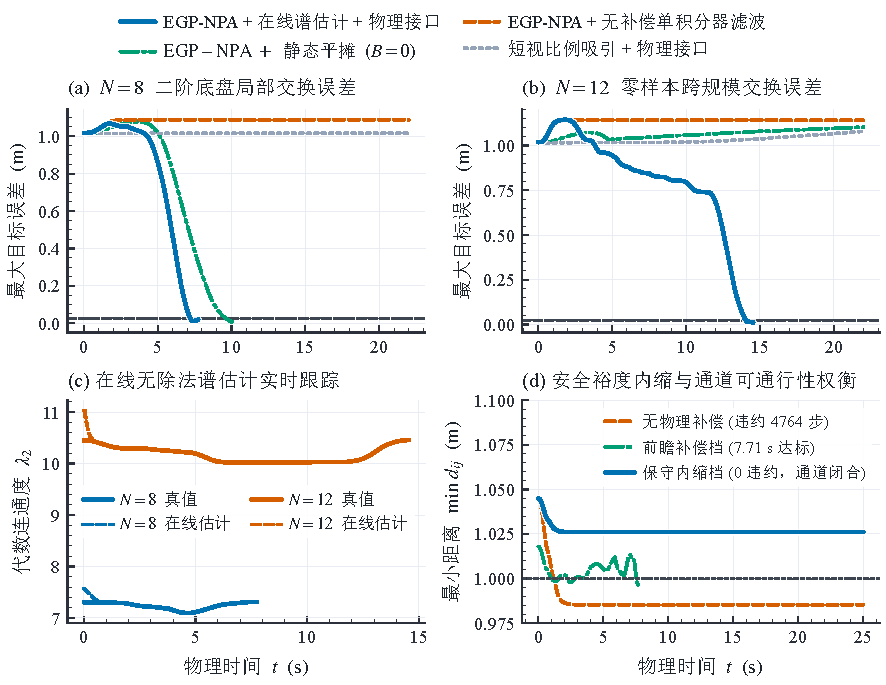
\includegraphics[width=\textwidth]{figures_zh/fig6_mujoco_verification.pdf}
 \caption[密集格点死锁下全栈 EGP-NPA + 在线谱估计 + 闭邻域 NPA 的 MuJoCo 闭环验证与权衡分析]{密集格点死锁下全栈 EGP-NPA + 在线无除法谱估计 + 闭邻域 NPA 的 \texttt{MuJoCo} 二阶全向底盘闭环验证。(a)--(b) 档位 A 下 $N=8$ 与 $N=12$ 局部交换任务的最大目标位置误差收敛曲线；(c) 在线无除法三通道谱估计器在物理闭环中的实时 $\hat{\lambda}_2(t)$ 跟踪表现；(d) 无物理补偿（\texttt{Ideal-NPA}）、前瞻补偿档（档位 A）与保守内缩档（档位 B）在最小机间净空 $\min d_{ij}(t)$ 与通道可通行性之间的实测权衡对比。}
 \label{fig:mujoco}
\end{figure*}

在二阶物理底盘中，为补偿速度环制动惯性引入物理安全距离内缩量 $\Delta d_{\mathrm{phys}}>0$（即将等效避碰距离由 $\ds$ 扩大至 $\ds^{\mathrm{phys}}=\ds+\Delta d_{\mathrm{phys}}$）时，存在如下关于密集格点通道可通行性的基本几何界限。

\begin{theorem}[二阶底盘物理安全裕度内缩下的密集通道闭合临界条件]\label{thm:passability-tradeoff}
设 $N$ 台机器人在初始格点间距为 $S>\ds$ 的平面三角晶格上执行位置互换任务。记外围阻挡邻居 $j,m$ 受限于全局连通半径或外层节点约束所能张开的最大横向通道孔径为 $d_{jm}^{\max}$。在物理收紧安全集 $\mathcal S^{\mathrm{phys}}=\{\bp\in\mathbb R^{2N}:\min_{a<b}d_{ab}\ge\ds+\Delta d_{\mathrm{phys}}\}$ 下：
\begin{enumerate}
 \item \textbf{初始静态可行性边界：} 初始晶格位于 $\operatorname{int}(\mathcal S^{\mathrm{phys}})$ 当且仅当 $\Delta d_{\mathrm{phys}}<S-\ds$；
 \item \textbf{三体接触膨胀下的通道拓扑闭合：} 当两台相向对穿的移动机器人 $i_1,i_2$ 同时穿过由外围邻居 $j,m$ 界定的孔径 $d_{jm}^{\max}$ 时，在对称交会中点处维持四机两两距离不小于 $\ds^{\mathrm{phys}}$ 要求四机构成边长至少为 $\ds^{\mathrm{phys}}$ 的接触菱形，所需最小横向孔径为 $d_{jm}^{\mathrm{req}}(\Delta d_{\mathrm{phys}})=\sqrt{3}(\ds+\Delta d_{\mathrm{phys}})$。一旦制动裕度满足 $\Delta d_{\mathrm{phys}}>d_{jm}^{\max}/\sqrt{3}-\ds$，交会通道在 $\mathcal S^{\mathrm{phys}}$ 中发生拓扑闭合（Topological Pinch-Off），初始构型与目标置换构型属于 $\mathcal S^{\mathrm{phys}}$ 的不同道路连通分支，任何保持 $\mathcal S^{\mathrm{phys}}$ 前向不变的连续轨迹均必然在通道入口处停滞。
\end{enumerate}
\end{theorem}
\begin{proof}
（1）由初始三角晶格最小机间距离 $\min_{a<b}d_{ab}(0)=S$ 直接得 $S>\ds+\Delta d_{\mathrm{phys}}\Longleftrightarrow\Delta d_{\mathrm{phys}}<S-\ds$。（2）在对称交会中点处，对穿节点 $i_1,i_2$ 间距满足 $d_{i_1 i_2}\ge\ds^{\mathrm{phys}}$，且各自到通道两侧节点 $j,m$ 的距离满足 $d_{i_1 j},d_{i_1 m},d_{i_2 j},d_{i_2 m}\ge\ds^{\mathrm{phys}}$。由平面菱形几何关系，两对角线长度满足 $(d_{i_1 i_2}/2)^2+(d_{jm}/2)^2\ge(\ds^{\mathrm{phys}})^2$，代入 $d_{i_1 i_2}\ge\ds^{\mathrm{phys}}$ 即得 $d_{jm}\ge\sqrt{3}\ds^{\mathrm{phys}}=\sqrt{3}(\ds+\Delta d_{\mathrm{phys}})$。故当 $d_{jm}^{\max}<\sqrt{3}(\ds+\Delta d_{\mathrm{phys}})$ 时，交会截面在 $\mathcal S^{\mathrm{phys}}$ 中为空集，连接初态与置换目标的任意连续路径必在某时刻违反 $d_{ab}(t)\ge\ds+\Delta d_{\mathrm{phys}}$。
\end{proof}

表\ref{tab:mujoco}与图\ref{fig:mujoco}对比了 $N=8$ 与 $N=12$ 共 $8$ 个高密度三角晶格任务在两档物理补偿参数下的 $64$ 次 \texttt{MuJoCo} 闭环运行结果：（1）如图\ref{fig:mujoco}(c) 所示，在线无除法谱估计器在约 $0.6\ \mathrm s$ 内收敛至真实代数连通度轨迹，全时域 RMSE 仅为 $0.0255\sim 0.0438$（相对误差低于 $0.5\%$），将在线估计值 $\hat\lambda_{2,i,k}$ 直接替代精确谱输入图网络节点特征后，全部 $64$ 次运行均实现 $0$ 步连通违约；（2）在优先保持通道机动性的前瞻补偿档（档位 A，初始间距 $S=1.018\ \mathrm m$）下，短视控制与无补偿滤波器到达率均为 $0/8$，静态平摊（$B=0$）仅到达 $1/8$，而全栈 EGP-NPA 在 $N=8$ 上实现 $3/4$ 到达、在 $N=12$ 零样本跨规模局部交换上实现到达（图\ref{fig:mujoco}(a)--(b)），并将平均终端误差压低至 $0.629\ \mathrm m$ 与 $1.314\ \mathrm m$；（3）正如定理\ref{thm:passability-tradeoff}所预言，在初始间隙仅 $1.8\sim 4.5\ \mathrm{cm}$ 的极限密集格点中，档位 A 下 $6.0\ \mathrm{kg}$ 车体的制动惯性会导致瞬态距离擦碰软边界（最低 $0.899\ \mathrm m\approx 2r_{\mathrm{body}}$），而当在档位 B（$S=1.045\ \mathrm m$）中施加 $\Delta d_{\mathrm{phys}}=0.028\ \mathrm m$ 保守距离内缩与 $\Delta u_{\max}=0.22\ \mathrm{m/s}$ 摆率限幅时，碰撞违约步数立即降为 $0$（图\ref{fig:mujoco}(d) 蓝色实线），但等效直径扩大 $2.8\%$ 直接触发三体交会通道几何闭合，使所有方法到达率均降为 $0/8$。这一结果客观界定了二阶物理系统在密集穿插任务中的工程适用条件：初始部署间距 $S$ 必须预留大于二阶制动包络 $\Delta d_{\mathrm{phys}}$ 的几何通行余量。
